
\chapter{Functions (2 of 2)}

Like many things in life, writing functions is best learned by example. This
chapter will feature several more of them that you can learn from and imitate.

\subsubsection{Basketball scoring: \texttt{bb\_pts()}}

Continuing the sports theme, the total points a basketball player scores is
related to the number of shots she makes of various kinds. Typically, the ``box
score'' of a game (see example in Figure~\ref{boxScore}) reports three scoring
stats: (1) the \textit{total} number of ``field goals''\footnote{A ``field
goal'' in basketball just means ``a regular basket'' -- \textit{i.e.}, not a
free throw penalty shot.} a player made and attempted, (2) the number of these
field goals, if any, that were for three points\footnote{In most leagues, a
basket is worth 2 points unless the shooter was farther than a certain distance
from the hoop when she shot it, in which case it's worth 3.}, and (3) the
number of free throws (``easy'' penalty shots) the player attempted and made.

Confusingly, (1) \textit{includes} (2). In other words, if the first number is
4 and the second is 1, the player didn't score 4 regular two-point baskets and
1 three-pointer, but rather \textit{3} two-point baskets and 1 three-pointer.

\begin{figure}[ht]
\centering
\fbox{
\mbox{
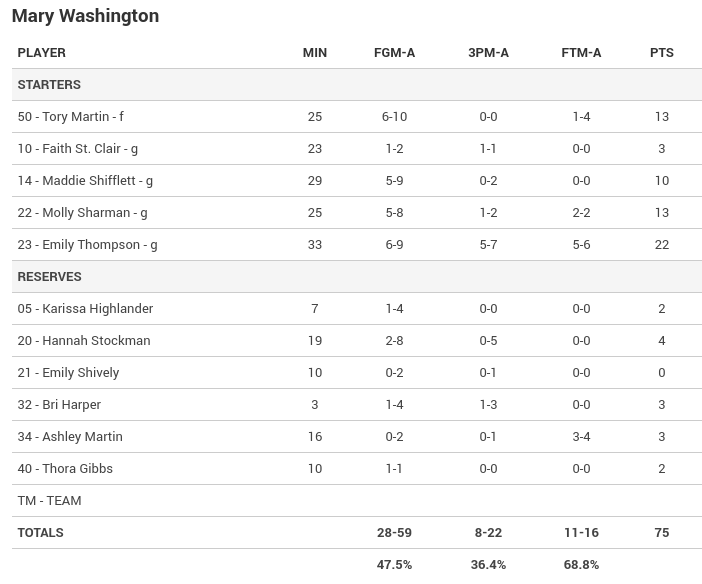
\includegraphics[width=0.8\textwidth]{boxScore.png}
}
}
\medskip
\caption{A basketball box score.}
\label{boxScore}
\end{figure}

In Figure~\ref{boxScore}, the \textsf{FGM-A} column gives the first of these
three categories, \textsf{3PM-A} the second, and \textsf{FTM-A} the third. The
\textsf{PTS} column gives the total number of points that player scored. (For
example, Molly Sharman made 5 of her 8 attempted field goals, one of which was
for three points, and she also converted both free throw attempts.)

All that took a lot longer to explain than the corresponding Python function:

\index{bb\_pts@\texttt{bb\_pts()}}

\begin{Verbatim}[fontsize=\footnotesize,samepage=true,frame=single,framesep=3mm]
def bb_pts(fgm, threep_fgm, ftm):
    return ((fgm - threep_fgm) * 2) + (threep_fgm * 3) + ftm

torys_pts = bb_pts(6, 0, 1)
print("Tory scored {} points.".format(torys_pts))
print("Emily scored {} points.".format(bb_pts(6,5,5)))
print("Lady Eagles scored {} points!".format(bb_pts(28,8,11)))
\end{Verbatim}
\vspace{-.2in}

\begin{Verbatim}[fontsize=\small,samepage=true,frame=leftline,framesep=5mm,framerule=1mm]
Tory scored 13 points.
Emily scored 22 points.
Lady Eagles scored 75 points!
\end{Verbatim}

\index{PEMDAS}

Strictly speaking you don't need all those bananas (regular PEMDAS
order-of-operations applies) but I think it's a good idea to include them for
clarity and grouping.

\subsubsection{``Exceptions'': \texttt{mean\_no\_outliers()} and \texttt{quiz\_avg()}}

Sometimes we want to take the straight average of a data set, but other times
we may want to filter out any strange or exceptional cases. Let's say we're
computing the average age of a classroom of college students, but we want to
remove any adult learners over 30 since that would skew the result. We could do
this sort of thing with a function like this:

\index{mean\_no\_outliers@\texttt{mean\_no\_outliers()}}
\index{low\_cutoff@\texttt{low\_cutoff}}
\index{high\_cutoff@\texttt{high\_cutoff}}

\begin{Verbatim}[fontsize=\footnotesize,samepage=true,frame=single,framesep=3mm]
def mean_no_outliers(a, low_cutoff, high_cutoff):
    return a[(a >= low_cutoff) & (a <= high_cutoff)].mean()

our_class = np.array([20,18,19,18,22,21,76,20,22,22,21,18])
print("The average age (excluding outliers) is {}.".format(
    mean_no_outliers(our_class, 0, 30)))
\end{Verbatim}

\vspace{-.2in}

\begin{Verbatim}[fontsize=\small,samepage=true,frame=leftline,framesep=5mm,framerule=1mm]
The average age (excluding outliers) is 20.09090909090909.
\end{Verbatim}

We've provided two arguments to the function besides the data set itself: a
lower and upper bound. Anything falling outside that range will be filtered
out. In the example function call, we passed 0 for the \texttt{low\_cutoff}
since we didn't desire to filter anything at the low end. (If we wanted to,
say, also remove children from the data set, we could have set that to 16 or
so.)

By the way, you might find the number of decimal places printed to be
unsightly. If so, we could enhance our function by rounding the result to (say)
two decimals with NumPy's \texttt{round()} function:

\index{round@\texttt{round()} function (NumPy)}
\label{round}

\begin{Verbatim}[fontsize=\footnotesize,samepage=true,frame=single,framesep=3mm]
def mean_no_outliers(a, low_cutoff, high_cutoff):
    return np.round(a[
        (a >= low_cutoff) & (a <= high_cutoff)].mean(),2)

print("The average age (excluding outliers) is {}.".format(
    mean_no_outliers(our_class, 0, 30)))
\end{Verbatim}
\vspace{-.2in}

\begin{Verbatim}[fontsize=\small,samepage=true,frame=leftline,framesep=5mm,framerule=1mm]
The average age (excluding outliers) is 20.09.
\end{Verbatim}

At this point you might think this function is getting pretty big for a
one-liner. I agree. Let's split it up and use some temporary variables to make
it more readable:

\begin{Verbatim}[fontsize=\footnotesize,samepage=true,frame=single,framesep=3mm]
def mean_no_outliers(a, low_cutoff, high_cutoff):
    filtered_data = a[(a >= low_cutoff) & (a <= high_cutoff)]
    filtered_average = np.round(filtered_data)
    return np.round(filtered_average,2)
\end{Verbatim}

Much clearer!

\medskip

A related but different example would be to remove a fixed \textit{number} of
data points from the end, instead of data points outside a specified range. For
instance, in my classes, I often give students (say) eight quizzes during a
semester, and drop the lowest two scores. That could be done with:

\index{sorting@sorting (arrays)}
\index{sort@\texttt{np.sort()} (NumPy)}
\index{quiz\_avg@\texttt{quiz\_avg()}}
\index{Filbert}

\begin{Verbatim}[fontsize=\footnotesize,samepage=true,frame=single,framesep=3mm]
def quiz_avg(quizzes):
    dropped_lowest_two = np.sort(quizzes)[2:]
    return dropped_lowest_two.mean()

filberts_quizzes = np.array([7,9,10,7,0,8,4,10])
print("Filbert's avg score was {}.".format(quiz_avg(
    filberts_quizzes)))
\end{Verbatim}
\vspace{-.2in}

\begin{Verbatim}[fontsize=\small,samepage=true,frame=leftline,framesep=5mm,framerule=1mm]
Filbert's avg score was 8.5.
\end{Verbatim}

Filbert's 0 and 4 were dropped, leaving him with a pretty good semester score.

The trick to this implementation is \textit{sorting} the quiz scores. Once you
do that, it's easy to pick out the top six to take the average, since the
lowest two scores will be at the beginning of the (sorted) array. Two notes
here:


\begin{compactitem}

\item We use the \texttt{np.sort()} function, not the \texttt{.sort()} method,
since we don't want to permanently change the order of \texttt{quizzes}. We
only need a temporarily sorted copy so we can omit the lowest two entries.

\index{slice}
\index{boxies (square brackets)}
\index{[]@\texttt{[]} (boxies)}

\item That business in the boxies (``\texttt{[2:]}'') is a \textbf{slice}
(recall section~\ref{slice} on p.~\pageref{slice}) which says ``only give me
entries number 2 through the end of the array.'' And that's exactly what the
doctor ordered to omit the first two.
\end{compactitem}

\smallskip

\subsubsection{Searching for values: \texttt{any\_zeros()}}

I'll end this chapter with an example which, like the ``preferred language''
example on p.~\pageref{spanishFrenchPitfall}, flummoxes nearly every beginning
student.

Suppose students in a DATA 101 course are given labs to complete, each one
worth up to 20 points. (This is purely hypothetical, as you can see.) At the
midway point of the semester, the instructor would like a quick list of any
students who failed to turn in one of the labs, so he can harass them for their
own good.

\index{Filbert}
\index{Betty Lou}
\index{Jezebel}
\index{Biff}
\index{Melvin}
\index{gradebook@\texttt{gradebook}}

Here's the \texttt{gradebook} \texttt{DataFrame} this professor is using:

\begin{Verbatim}[fontsize=\footnotesize,samepage=true,frame=leftline,framesep=5mm,framerule=1mm]
           Q1  Q2  Q3  Q4  lab1  lab2  lab3  lab4  lab5
student                                                
Filbert     7   9  10   7    15    19    14    20    20
Jezebel     8   7   0   6    12    12    16     0    20
Betty Lou  10  10  10  10    20    20    20    20    20
Biff        3   2   6   5    10    12     0     0    16
Melvin      0   0  10  10     0    18    20    14    20
\end{Verbatim}

\index{print\_harass\_list@\texttt{print\_harass\_list()}}

Let's write a function called \texttt{print\_harass\_list()} whose job is to
tell this professor which students he should check up on. We'll write it as
follows:

\begin{Verbatim}[fontsize=\footnotesize,samepage=true,frame=single,framesep=3mm]
def print_harass_list(gradebook):
    for row in gradebook.itertuples():
        if any_zeros(np.array([row.lab1, row.lab2, row.lab3,
            row.lab4, row.lab5])):
            print("Better check up on {}.".format(row.Index))
\end{Verbatim}

\index{iteration}

\index{any\_zeros@\texttt{any\_zeros()}}
Note that we've pushed some of the work on to a new function,
\texttt{any\_zeros()}, that we haven't written yet. This is good organizational
style. Now \texttt{print\_harass\_list()} can do the job of iterating through
the \texttt{DataFrame} rows, extracting the lab scores, and printing a message
if necessary, whereas it defers to \texttt{any\_zeros()} to inspect the lab
scores and determine the presence of any zeros.

It doesn't work until we actually write the second function, of course, so here
goes. Heads up, since this is the part that perplexes students. The following
implementation of \texttt{any\_zeros()} looks perfectly reasonable, yet is dead
WRONG:

\begin{Verbatim}[fontsize=\small,samepage=true,frame=single,framesep=3mm]
def any_zeros_WRONG(labs):
    for lab in labs:
        if lab == 0:
            return True
        else:
            return False
\end{Verbatim}

It looks so correct! And yet it is not. Check out the result:

\begin{Verbatim}[fontsize=\small,samepage=true,frame=single,framesep=3mm]
print_harass_list(gradebook)
\end{Verbatim}
\vspace{-.2in}

\begin{Verbatim}[fontsize=\small,samepage=true,frame=leftline,framesep=5mm,framerule=1mm]
Better check up on Melvin.
\end{Verbatim}

Clearly we need to check up on \texttt{Jezebel} and \texttt{Biff} as well (look
at their scores for labs 3 and 4), yet they inexplicably didn't get printed.

\index{cardinal rule@cardinal rule (of \texttt{if}/\texttt{else})}

Here's what's WRONG with that \texttt{any\_zeros()} attempt. Stare carefully at
that loop and realize that the \textit{body} of the loop is comprised of a
single \texttt{if}/\texttt{else} statement. And remember our cardinal rule from
the grey box on p.~\pageref{cardinalRule}: either the \texttt{if} body or the
\texttt{else} body will \textit{always} be executed.

That means that this loop is destined to only execute exactly once! It doesn't
matter how long the \texttt{labs} array is. It effectively looks only at the
\textit{first} element, and decides based solely on that whether or not the
entire array has any zeros in it!

\index{any\_zeros@\texttt{any\_zeros()}}
The correct version of \texttt{any\_zeros()} would look like this:

\begin{Verbatim}[fontsize=\small,samepage=true,frame=single,framesep=3mm]
def any_zeros(labs):
    for lab in labs:
        if lab == 0:
            return True
    return False
\end{Verbatim}

\index{indentation}

At first glance, it may appear unchanged, but look again. First of all, there's
no \texttt{else} anymore. Second of all, the ``\texttt{return False}'' line is
indented \textit{evenly with the word \texttt{for}}. This means that
``\texttt{return False}'' is \textit{not} part of the loop at all: it will only
run \textit{after} the entire loop has executed.

That turns out to make all the difference. The function will dutifully go
through \textit{each} element of the \texttt{labs} array, inspecting each one
to see whether it's zero. As soon as it finds a zero, it returns \texttt{True},
since then its job is done. Only after inspecting the \textit{entire} array,
and coming up empty on its zero quest, does this function then have the
audacity to return \texttt{False}, meaning ``nope! Clean as a whistle.'' The
result:

\begin{Verbatim}[fontsize=\small,samepage=true,frame=leftline,framesep=5mm,framerule=1mm]
Better check up on Jezebel.
Better check up on Biff.
Better check up on Melvin.
\end{Verbatim}

\subsubsection{Postlude: thinking algorithmically}

\index{algorithmic thinking}
\index{holistic thinking}
\index{thinking algorithmically vs.~holistically}

Getting tripped up on that last example is, I believe, usually a case of
\textit{thinking holistically} rather than \textit{thinking algorithmically}.
Math classes have trained people to think holistically, by which I mean looking
at (say) a bunch of equations and viewing them as ``all equally true, all at
once.'' And this is the correct way to think mathematically. If I give you five
simultaneous equations that state relationships among variables, they aren't
really in any order. They're just ``five true things.''

But programming requires you to think algorithmically. You have to execute the
code in your head, step by step, and realize the consequences. The appealing
symmetry of the WRONG \texttt{any\_zeros()} function is appealing because
you're looking at it as a whole: ``it's looping (seemingly) through all the
elements, with zeros being an indicator of \texttt{True}ness and non-zeros
being an indicator of \texttt{False}ness. What's not to like?'' The error, as
you saw, is that when running through the data step-by-step, there are immense
ramifications of returning early. That's only apparent if you think of the code
executing sequentially as it goes. You have to pretend you're the computer, not
a mathematician.

% Other examples:
% def is_tall(ht_ft, ht_in, sex):
%    inches_tall = ht_ft * 12 + ht_in
%    if sex == "male":
%        if inches_tall > 70:
%            return True
%        else:
%            return False
%    else:
%        if inches_tall > 64:
%            return True
%        else:
%            return False
